\section*{Introducción}

Las células dendríticas epidérmicas conocidas como \et{células de Langerhans} (CL) desempeñan un papel determinante en el desarrollo de la respuesta inmune, ya que tiene como función la detección, transporte y presentación de antígenos a los linfocitos B vírgenes, los cuales se encargan de llevar a cabo la respuesta inmune adaptativa\cite{article:CL}.

Las CL se localizan en la capa más externa de la piel la epidermis, su identificación es realizada por medio microscopía óptica en muestras de piel procesadas con tinciones histológicas especializadas, donde se observa su morfología celular, la cual consta de un soma de contorno irregular del cual proceden prolongaciones alargadas que le dan forma estrellada.

Se han realizados estudios en piel de mamíferos contribuyendo a su caracterización y análisis, sin embargo las técnicas disponibles no son capaces de la identificación de forma general definir CL en todos los vertebrados, el estudio de CL en \et{vertebrados no mamíferos} es un paso para la integración de la respuesta innata y adaptativa \cite{article:vertebrados}, debido a la disponibilidad, existencia y elevado precio de reactivos e instrumentos el estudio de CL en vertebrados no mamíferos se ve reducido.

Las impregnaciones metálicas son técnicas de tinción que se basan en reacciones de precipitación, en las cuales se presentan interacciones atractivas del producto de reacción con la superficie celular de una o más células de forma específica en un tejido, las \et{impregnaciones yoduro de zinc-tetróxido de osmio} (ZIO) \cite{article:ZIO} y \et{cloruro de oro} \cite{article:ClAu} han sido empleadas en la identificación de CL en mamíferos Figura 1 y 2, las condiciones de reacción tienden a ser poco definidas, y han caido en desuso pese a buenos resultados que se obtienen.

\begin{figure}[h]
    \begin{minipage}[b]{0.225\textwidth}
        \centering
        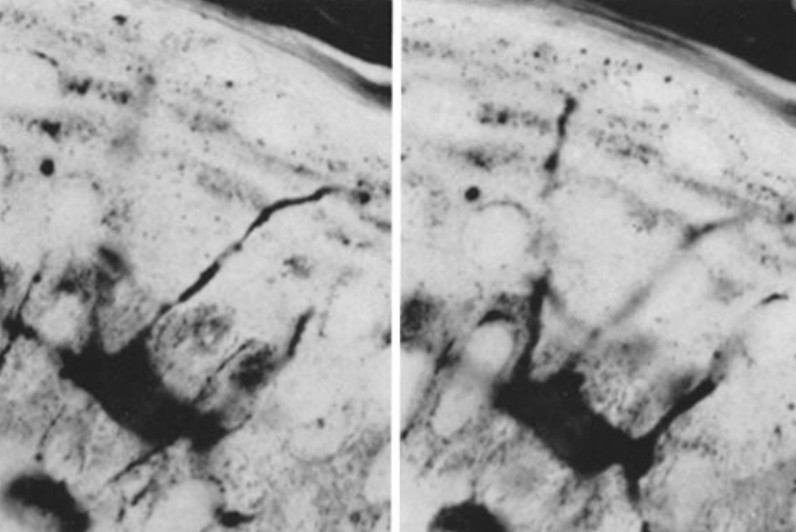
\includegraphics[scale=0.2325,frame]{ImpregancionZIO.jpg}
        \caption{\small{CL en piel de humano con la impregnación ZIO.}}
    \end{minipage}
    \hfill
    \begin{minipage}[b]{0.25\textwidth}
        \centering
        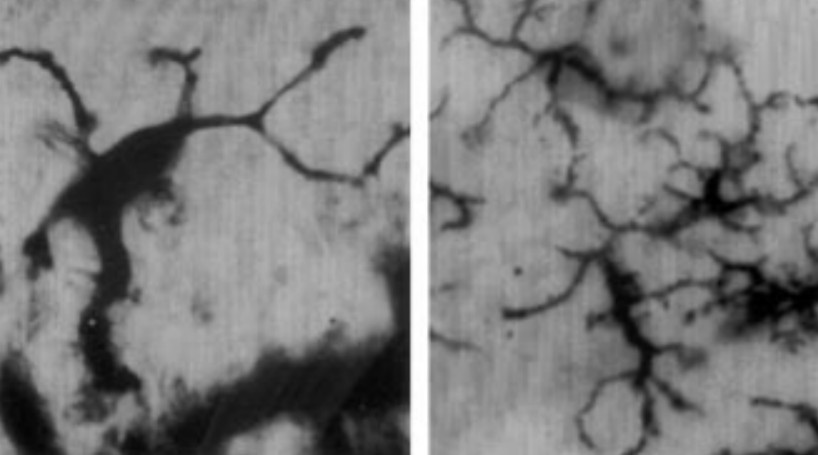
\includegraphics[scale=0.2725,frame]{ImpregancionAu.jpg}
        \caption{\small{CL en piel de humano con la impregnación de cloruro de oro.}}
    \end{minipage}
\end{figure}

Las técnicas ZIO y cloruro de oro no han sido empleadas en otros vertebrados que no sean mamíferos, pero se espera que la interacción entre el producto de reacción de dichas impregnaciones y las CL en vertebrados no mamíferos sea favorable, debido al parecido en la composición de su superficie celular.

El analizar las impregnaciones ZIO y cloruro de oro como técnicas capaces de la identificación de CL, definir las condiciones óptimas de reacción y  compararla con una técnica confiable como la \et{histoquímica enzimática} para ATPasa\cite{article:ATPasa}, lo cual proveerá técnicas específicas, confiables y repetibles para el estudio de las CL en los vertebrados no mamíferos.